\section{Introduction}

\subsection{History}

\begin{frame}{History}
    \begin{itemize}[label=$\star$]
        \item The \textbf{Trie} data structure was first introduced by \textbf{René de la Briandais} in 1959 as an efficient method
for storing and retrieving strings in a lexicon
        \item It was later independently developed by \textbf{Edward
Fredkin} in 1960.
    \begin{figure}[h]
    \centering
    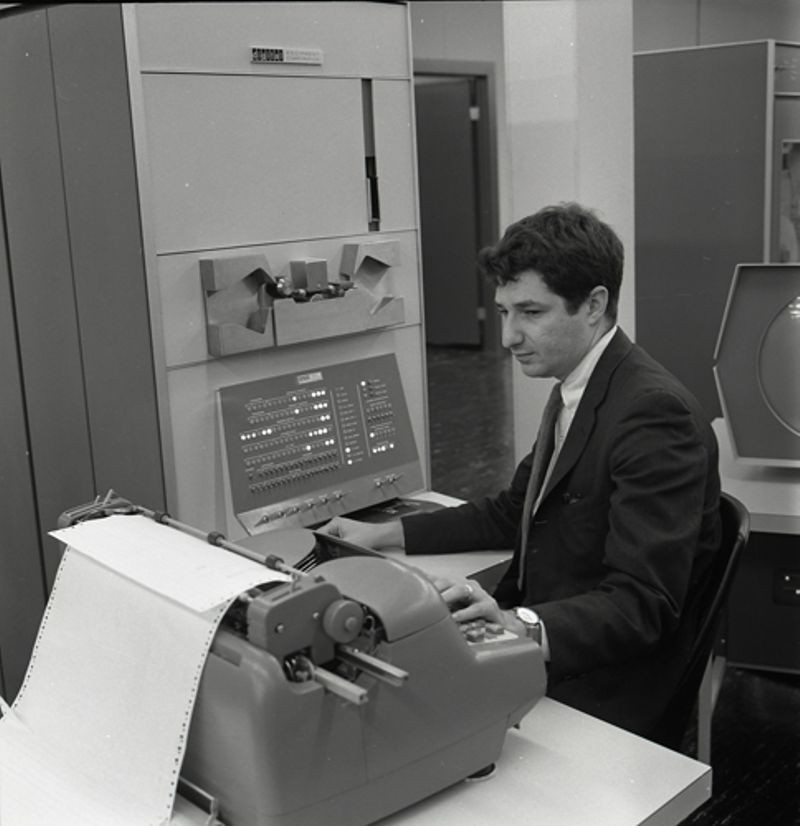
\includegraphics[scale=0.15]{EdSemi.jpg}
    \caption{Edward Fredkin}
    \label{fig:edsemi}
\end{figure}
    \end{itemize}
\end{frame}
\subsection{Definition}
\begin{frame}{Definition}
\textbf{A Trie} (also known as a \textbf{prefix tree}) is a tree-like data structure used to store a dynamic set or associative array where the keys are usually strings.
\begin{figure}[h]
    \centering
    \begin{tikzpicture}[scale=0.6]
        % Vẽ hình elips chứa "Root node" tại tọa độ (0,0)
        \node[ellipse, draw, minimum width=2cm, minimum height=1cm] at (1,0) {Root node};
        
        % Vẽ vòng tròn chứa "a" tại (0,-2), không tô màu
        \fill[green] (0,-5) circle (0.5cm);
        \draw (0,-2) circle (0.5cm);
        \node at (0,-2) {\textbf{a}}; % Chữ "a" in đậm ở tâm vòng tròn
        \draw[->] (1,-0.8) -- (0,-1.5); % Mũi tên từ dưới "Root node" tới trên "a"
        
        % Vẽ vòng tròn chứa "p" thứ nhất tại (0,-3.5), không tô màu
        \draw (0,-3.5) circle (0.5cm);
        \node at (0,-3.5) {\textbf{p}}; % Chữ "p" in đậm ở tâm vòng tròn
        \draw[->] (0,-2.5) -- (0,-3); % Mũi tên từ dưới "a" tới trên "p"
        
        % Vẽ vòng tròn chứa "p" thứ hai tại (0,-5), không tô màu
        \draw (0,-5) circle (0.5cm);
        \node at (0,-5) {\textbf{p}}; % Chữ "p" in đậm ở tâm vòng tròn
        \draw[->] (0,-4) -- (0,-4.5); % Mũi tên từ dưới "p" trước tới trên "p"
        
        % Vẽ vòng tròn chứa "l" tại (0,-6.5), không tô màu
        \draw (0,-6.5) circle (0.5cm);
        \node at (0,-6.5) {\textbf{l}}; % Chữ "l" in đậm ở tâm vòng tròn
        \draw[->] (0,-5.5) -- (0,-6); % Mũi tên từ dưới "p" tới trên "l"
        
        % Vẽ vòng tròn chứa "e" tại (0,-8), tô màu xanh dương
        \fill[green] (0,-8) circle (0.5cm); % Tô nền màu xanh dương
        \draw (0,-8) circle (0.5cm); % Vẽ viền vòng tròn
        \node at (0,-8) {\textbf{e}}; % Chữ "e" in đậm ở tâm vòng tròn
        \draw[->] (0,-7) -- (0,-7.5); % Mũi tên từ dưới "l" tới trên "e"

        % b
        \draw (2.75,-2) circle (0.5cm);
        \node at (2.75,-2) {\textbf{b}}; % Chữ "b" in đậm ở tâm vòng tròn
        \draw[->] (1,-0.8) -- (2.75,-1.5); % Mũi tên từ dưới "Root node" tới trên "b"
        % a
        \draw (2.75,-3.5) circle (0.5cm);
        \node at (2.75,-3.5) {\textbf{a}}; % Chữ "a" in đậm ở tâm vòng tròn
        \draw[->] (2.75,-2.5) -- (2.75,-3); % Mũi tên từ dưới "b" tới trên "a"
        % s
        \draw (3.5,-5) circle (0.5cm);
        \node at (3.5,-5) {\textbf{s}}; % Chữ "s" in đậm ở tâm vòng tròn
        \draw[->] (2.75,-4) -- (3.5,-4.5); % Mũi tên từ dưới "a" tới trên "s"
        % e
        \fill[green] (3.5,-6.5) circle (0.5cm);
        \draw (3.5,-6.5) circle (0.5cm);
        \node at (3.5,-6.5) {\textbf{e}}; % Chữ "e" in đậm ở tâm vòng tròn
        \draw[->] (3.5,-5.5) -- (3.5,-6); % Mũi tên từ dưới "s" tới trên "e"
        % t
        \fill[green] (2,-5) circle (0.5cm);
        \draw (2,-5) circle (0.5cm);
        \node at (2,-5) {\textbf{t}}; % Chữ "t" in đậm ở tâm vòng tròn
        \draw[->] (2.75,-4) -- (2,-4.5); % Mũi tên từ dưới "a" tới trên "t"
        % m
        \draw (2,-6.5) circle (0.5cm);
        \node at (2,-6.5) {\textbf{m}}; % Chữ "m" in đậm ở tâm vòng tròn
        \draw[->] (2,-5.5) -- (2,-6); % Mũi tên từ dưới "t" tới trên "m"
        % a
        \draw (2,-8) circle (0.5cm); % Vẽ viền vòng tròn
        \node at (2,-8) {\textbf{a}}; % Chữ "a" in đậm ở tâm vòng tròn
        \draw[->] (2,-7) -- (2,-7.5); % Mũi tên từ dưới "m" tới trên "a"
        % n
        \fill[green] (2,-9.5) circle (0.5cm); % Tô nền màu xanh dương
        \draw (2,-9.5) circle (0.5cm); % Vẽ viền vòng tròn
        \node at (2,-9.5) {\textbf{n}}; % Chữ "n" in đậm ở tâm vòng tròn
        \draw[->] (2,-8.5) -- (2,-9); % Mũi tên từ dưới "a" tới trên "n"
    \end{tikzpicture}
\end{figure}
   
\end{frame}
\subsection{Purpose}
\begin{frame}{Purpose}
   The primary purpose of a Trie is to efficiently handle dictionary operations like searching, insertion,and deletion of words. It is widely used in applications like autocomplete, spell checking, IP routing, and DNA equencing.
\end{frame}